\mainmatter
% Partie 1: présentation du personnage
\chapter{La Vie, le Jazz, le Verbe}\footnote{L'emploi de majuscules, ici,
n'est ni fortuit, ni une basse erreur typographique (Faustroll m'en préserve !). Ces trois mots ont été nomproprifiés (en utilisant un détergent du
meilleur tonneau, préservant les couleurs) à dessein et sans scrupule,
étant donné l'importance de ce qu'ils représentent avaient pour le sujet du
présent document.}
\epigraph{%
Je n'ai pas besoin de gagner ma vie, puisque je l'ai déjà.}{Boris Vian}
\vfill
\pagebreak
%\section{\BV, Bison \bsc{Ravi}, et tous leurs amis}
%\section{{\sout{Une}} Des vie{\uline{s}} bien remplie{\uline{s}}}
\section{Des vies bien remplies}
\epigraph{Romancier, poète, dramaturge, ingénieur, trompettiste, auteur
de chansons et de film, directeur artistique de maisons de disques, pataphysicien, roi
de Saint-Germain-des-Prés\ldots Ce sont bien mille et une vies que Boris Vian sera parvenu
à vivre en trente-neuf ans d'existence.}
{\emph{Les Vies parallèles de Boris Vian}, Noël \bsc{Arnaud}, quatrième de couverture}

% Intro

\lettrine{I}l est difficile de parler de \BV. Peut-être parce qu'il
est difficile de lui coller une seule étiquette. Un seul nom,
même. « \BV\ » pour l'état civil, « Bison \bsc{Ravi} » --- anagramme
de « \BV\ » pour les proches, « Vernon \bsc{Sullivan} » pour certains
livres, et des dizaines d'autres pseudonymes en tant que chroniqueur.
% TODO: lien liste des pseudonymes (annexes ?)
Mais pour évoquer le personnage, on peut déjà s'intéresser à l'Histoire,
et à son histoire.

% TODO: Annexe frise chrono ?

\subsection{Contexte historique}
Il est nécessaire de décrire le contexte historique de la vie
de \BV\ pour comprendre certaines forces externes qui
ont pu avoir une influence significative sur sa vie, ainsi que
sur son  \oe{}uvre.

\BV\ est né peu après la seconde guère mondiale. En \nb{1929}, c'est
la crise avec le crash de Wall Street. En \nb{1940}, l'Allemagne envahit la
partie nord de la France. Toute une partie de la culture est alors
interdite et censurée, notamment le jazz, d'origine noire-américaine.

\subsection{Famille et éducation}

\BV \ est issu d'une famille riche. Son père, Paul \bsc{Vian}, est rentier
depuis ses \nb{20} ans. Sa mère est l'héritière d'une riche famille de l'industrie
du papier.

Les Vian habitent une grande maison, «Les Fauvettes», à Ville d'Avray, dans la
banlieue de Paris, près du parc de Saint-Cloud. Le plus important est le loisir,
le divertissement, tout ce qui est agréable. Les enfants Vian vivent ainsi coupés
du monde extérieur: la politique, la religion, ou tout autre sujet sérieux n'entre
pas dans ce petit monde clos. On profite de la vie.

Cette maison n'est pas le seul paradis des Vian. Tous les étés, ils se rendent
à Landemer, dans le Cotentin, où les enfants peuvent jouer tout l'été sur la
plage privée de la propriété apportée par la famille de  M\up{me} \bsc{Vian}. 

\subsection{Les études}
Il n'y rien de bien passionnant à raconter de ses études. Collège, lycée, prépa, Centrale.
On peut tout de même parler de Centrale: au moment où il y étudie, celle-ci
se replie à Angoulême à cause de l'occupation. Il appartient à la promotion \nb{42}b.

Voilà pour son parcours\ldots Si l'on met les mots de Wolf, de \emph{L'herbe rouge},
dans la bouche de \BV\ (pourquoi pas, il a bien fait l'inverse ! Ce n'est donc qu'un
juste retour des choses), voilà ce que pense Boris de l'éducation:

{\small
\begin{quotation}
– Monsieur Brul, dit Wolf en martelant ses mots, écoutez ce que je vais vous répondre. Écoutez bien. Vos études, c’est de la blague. C’est ce qu’il y a de plus facile au monde. On essaye de faire croire aux gens, depuis des générations, qu’un ingénieur, qu’un savant, c’est un homme d’élite. Eh bien, je rigole ; et personne ne s’y trompe, – sauf les prétendus hommes d’élite eux-mêmes – Monsieur Brul, c’est plus difficile d’apprendre la boxe que les mathématiques. Sinon, il y aurait plus de classes de boxeurs que de classes de calcul dans les écoles. C’est plus difficile de devenir un bon nageur que de savoir écrire en français. Sinon, il y aurait plus de maîtres baigneurs que de professeurs de français. Tout le monde peut être bachelier, Monsieur Brul… et d’ailleurs, il y a beaucoup de bacheliers, mais comptez le nombre de ceux qui sont capables de prendre part à des épreuves de décathlon. Monsieur Brul, je hais mes études, parce qu’il y a trop d’imbéciles qui savent lire : et ces imbéciles ne s’y trompent pas, qui s’arrachent les journaux sportifs et glorifient les gens du stade. Et mieux vaudrait apprendre à faire l’amour correctement que de s’abrutir sur un livre d’histoire.

Monsieur Brul leva une main timide.

– Ce n’est pas moi qui dois vous questionner là-dessus, dit-il. Ne sortez pas du sujet, encore une fois.

– L’amour est une activité physique aussi négligée que les autres, dit Wolf.

– Possible, répondit Monsieur Brul, mais on lui consacre en général un chapitre spécial.

– Bon, dit Wolf, n’en parlons plus. Vous savez maintenant ce que j’en pense, de vos études. De votre gâtisme. De votre propagande. De vos livres. De vos classes puantes et de vos cancres masturbés. De vos cabinets pleins de merde et de vos chahuteurs sournois, de vos normaliens verdâtres et lunettards, de vos polytechniciens poseurs, de vos centraux confits dans la bourgeoisie, de vos médecins voleurs et de vos juges véreux… bon sang… parlez-moi d’un bon match de boxe… c’est truqué aussi, mais au moins ça soulage.
\end{quotation}
}

Une analyse rapide permet d'affirmer que pour l'auteur, les études représentent
une perte de temps. Non pas qu'elles sont inutiles, puisqu'elles mènent à un
travail, qui permet de gagner sa vie. Mais au pris de combien d'années de jeunesse,
qui passent pour ne pas revenir\ldots

\subsection{L'ingénieur}

\BV\ a l'esprit d'un ingénieur. Créatif, il trouve toujours
un moyen pour résoudre un problème. Inventif, aussi\~: il déposera
plusieurs brevets, dont un pour une roue souple. Imaginatif\footnote{Avec tous ces tifs,
il aurait aussi bien pu faire coiffeur\ldots}\~: le pianocktail de \emph{L'écume}
est une pure merveille, qui ravit tous les sens\~: il est beau, il sonne bien,
et fait des cocktails délicieux.

Au delà de son état d'esprit, il faut se rendre compte qu'une fois de plus,
il juge durement la société dans laquelle il vit. Le titre d'ingénieur, est,
pour lui un passeport --- ou, comme il aime à le dire, une «peau d'âne» ---, une
preuve de sérieux, pour avoir la légitimité de dire des bêtises. À nouveau on pourrait
citer \emph{L'herbe}, ou Wolf exprime l'opinion de Boris avec force, mais également
Boris lui-même. On a ainsi une vidéo où il explique --- en anglais, \emph{please} ---
à son intervieweuse, qui a du mal à suivre:

{\small
\begin{quotation}
- Combien de métiers avez-vous exercé ?

- J'ai d'abord été ingénieur, parce que je ne connaissais rien aux
mathématiques, comme l'italien, vous savez, donc je devais les étudier.
J'ai donc appris les mathématiques, et je suis devenu ingénieur.
C'était très pratique, voulant plus tard faire des choses stupides,
et il me fallait un diplôme pour le faire de manière convenable.

- Mais vous êtes devenu écrivain à la place.

- Non, j'ai d'abord été ingénieur, mais pendant mes heures de travail
j'avais\ldots disons\ldots du temps libre, que j'utilisais pour écrire.
\end{quotation}
}

Il en a effectivement fait es \emph{silly things}, durant ses heures de travail ! Il a
travaillé à l'AFNOR, à la rédaction de normes en tout genre. Comme exemple, se
référer à la fig. \ref{ins}, proposant une normalisation des insultes pour le français moyen.

Mais son «temps libre», à l'AFNOR d'abord puis à l'Office du papier, lui a permis aussi d'écrire ses premiers romans\~:
\emph{Vercoquin et le plancton} --- qui, au passage, ne manque pas de caricaturer l'AFNOR
et ses occupants --- et \emph{Trouble dans les Andains} pour ne citer qu'eux.

\begin{figure}
\centering
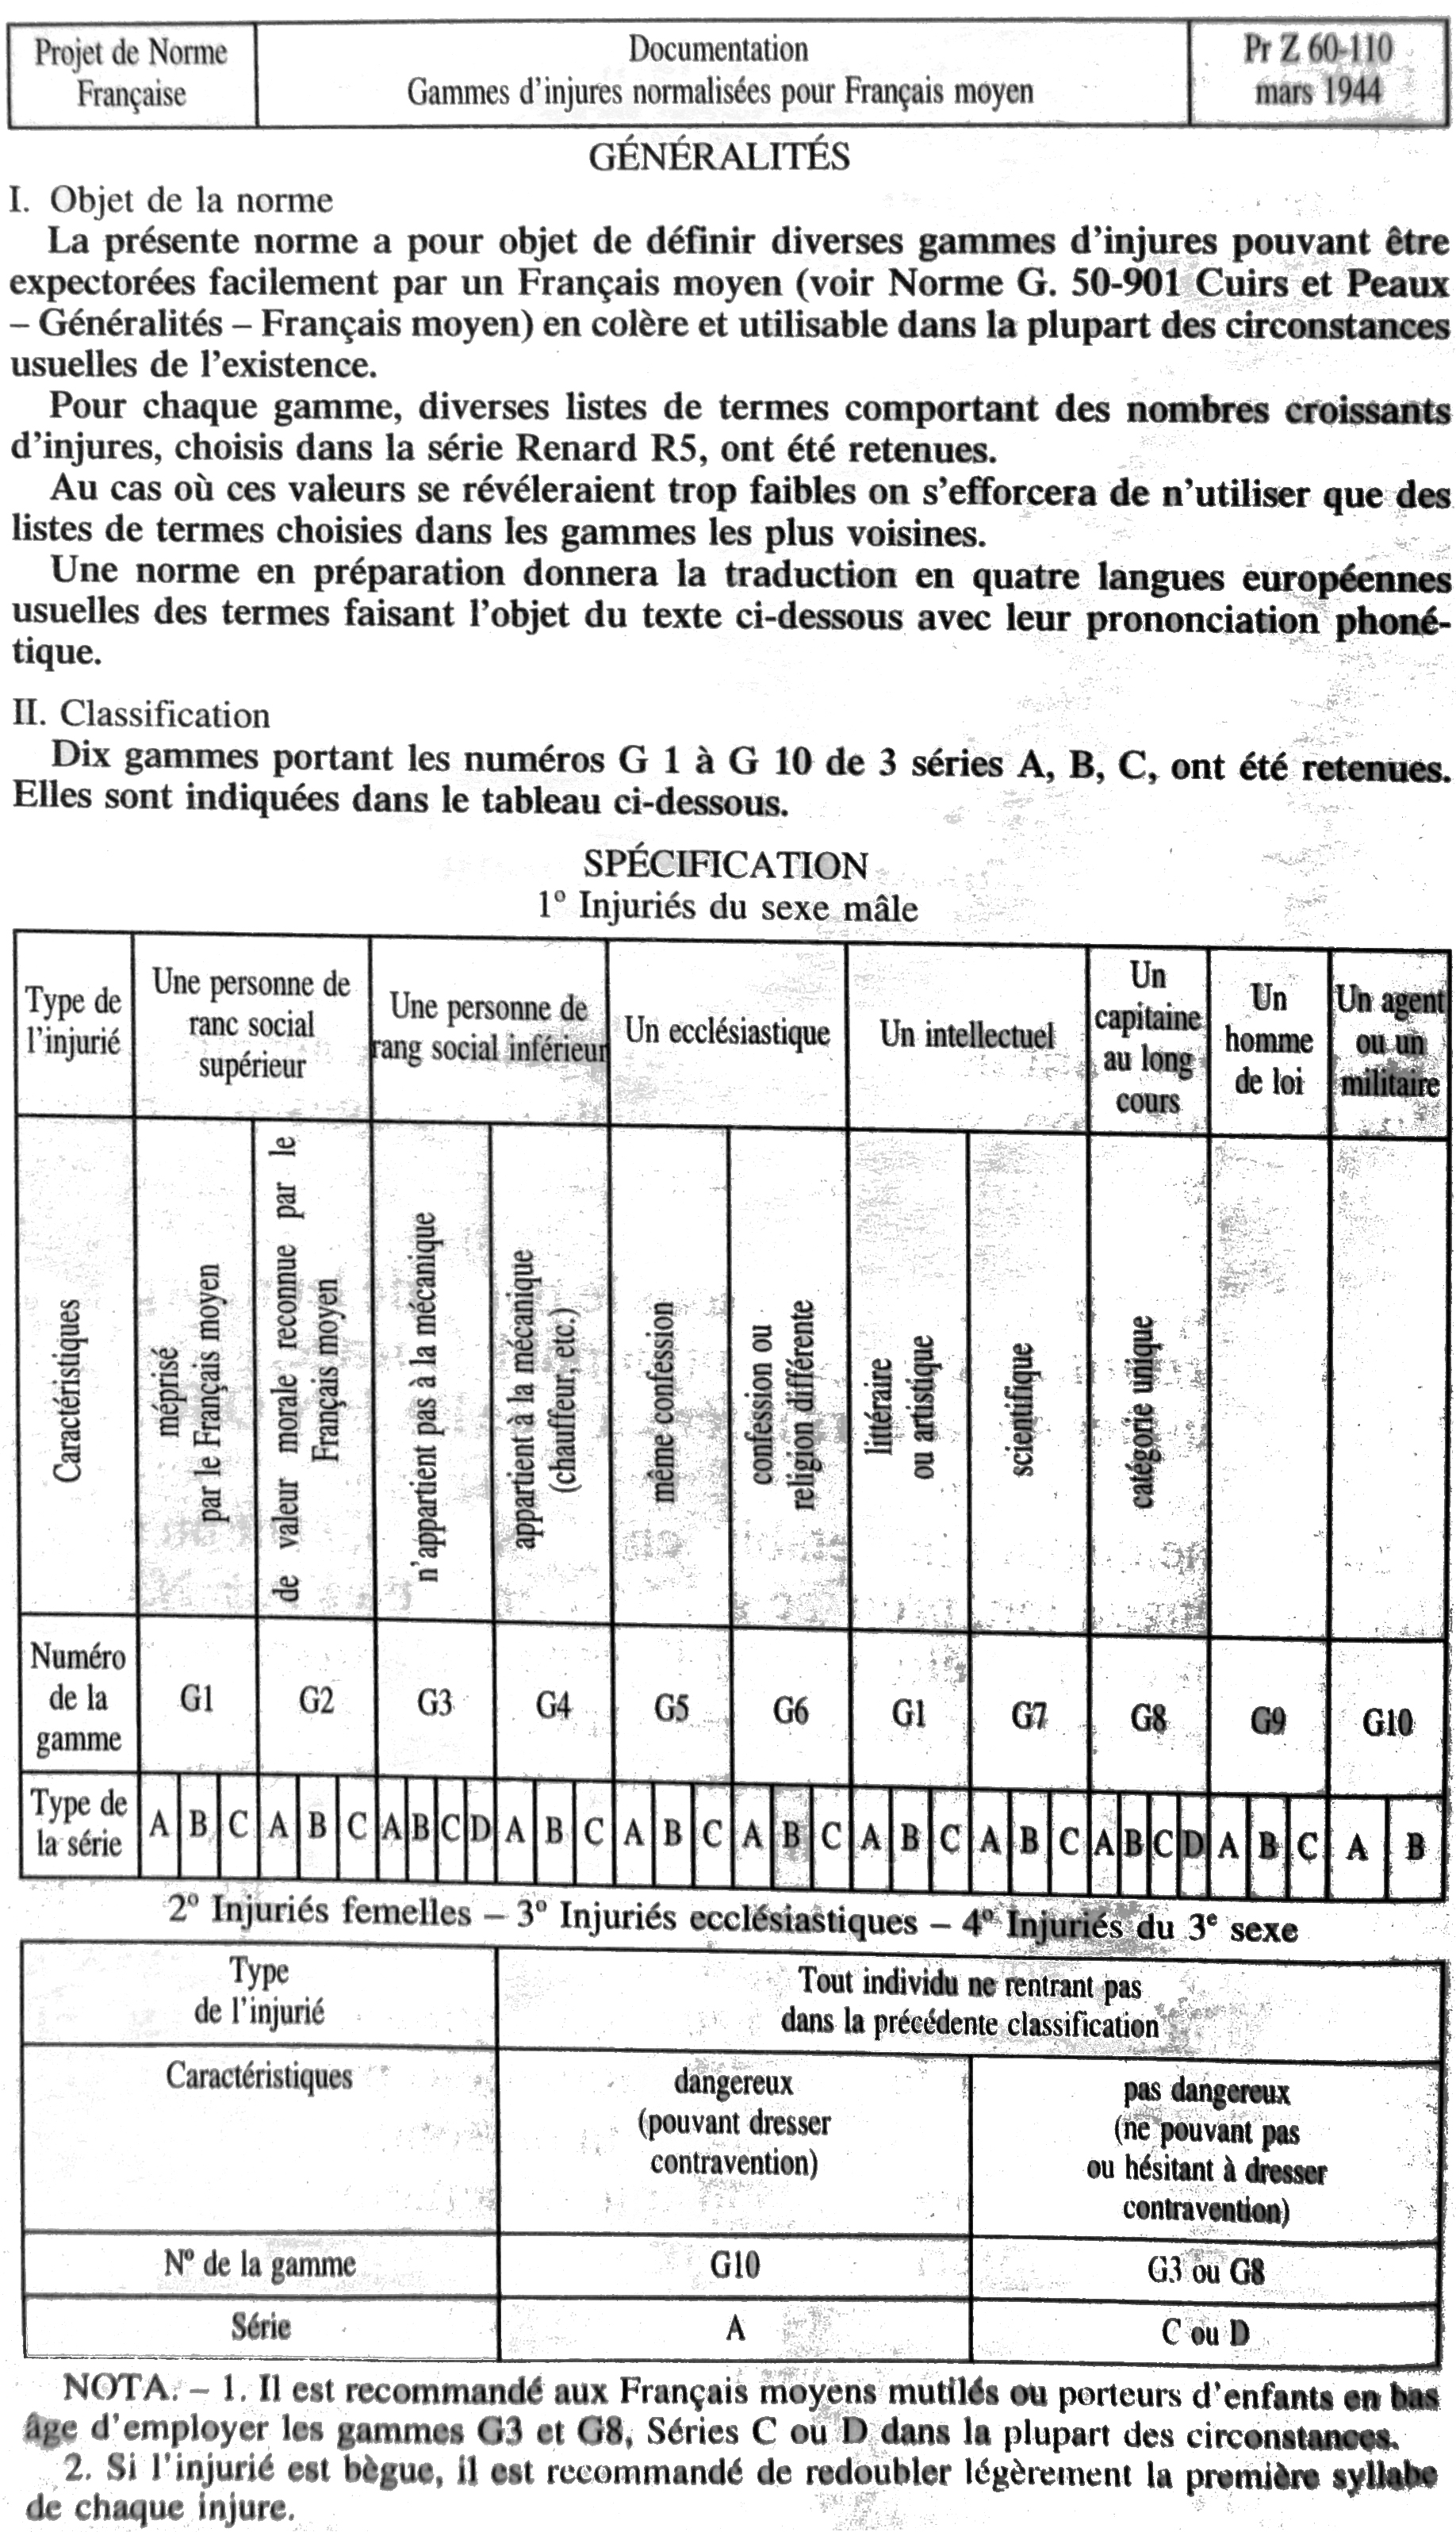
\includegraphics[height=\textheight]{\PIXPATH/ins}
\caption{Exemple de document rédigé à l'AFNOR}
\label{ins}
\end{figure}

\subsection{Le créateur}

\section{Le Jazz}
\epigraph{Il [\BV] était un amoureux du jazz, ne vivait que pour le jazz, n'entendait, ne s'exprimait qu'en jazz.}
{Henri Salvador}

S'il y a bien quelque chose de stable et présent à travers toute l'existence de \BV, c'est le jazz.
Amateur inconditionnel, joueur de trompinette, critique, directeur artistique: dès son adolescence, et
jusqu'à sa mort, le jazz a marqué sa vie à chaque instant. Rien que ce «fil» de sa vie mériterait
qu'on y consacre un ouvrage entier. Voilà quelques pistes pour analyser ce qui représentait
sa raison de vivre.

\subsection{L'amateur}

Il est d'abord amateur. C'est que ça swingue, chez les Vian et dans la jeunesse parisienne !
On se trémousse sur des rythmes de la Nouvelle Orléans, de la musique noire\ldots
S'inscrivant très tôt à l'alors très jeune Hot Club de France, il ne perd
pas une miette de l'évolution de ce genre en France. On peut même dire
qu'il l'encourage de toues ses forces, en particulier en jouant du jazz.

\subsection{Le musicien}

Il apprend à jouer de la trompette --- en fait une petite trompette qu'il appelle affectueusement «trompinette» ---,
au début à la manière de Bix \bsc{Beiderbecke}, puis, sous d'autres influences, développe
son style propre.

\begin{figure}
\centering
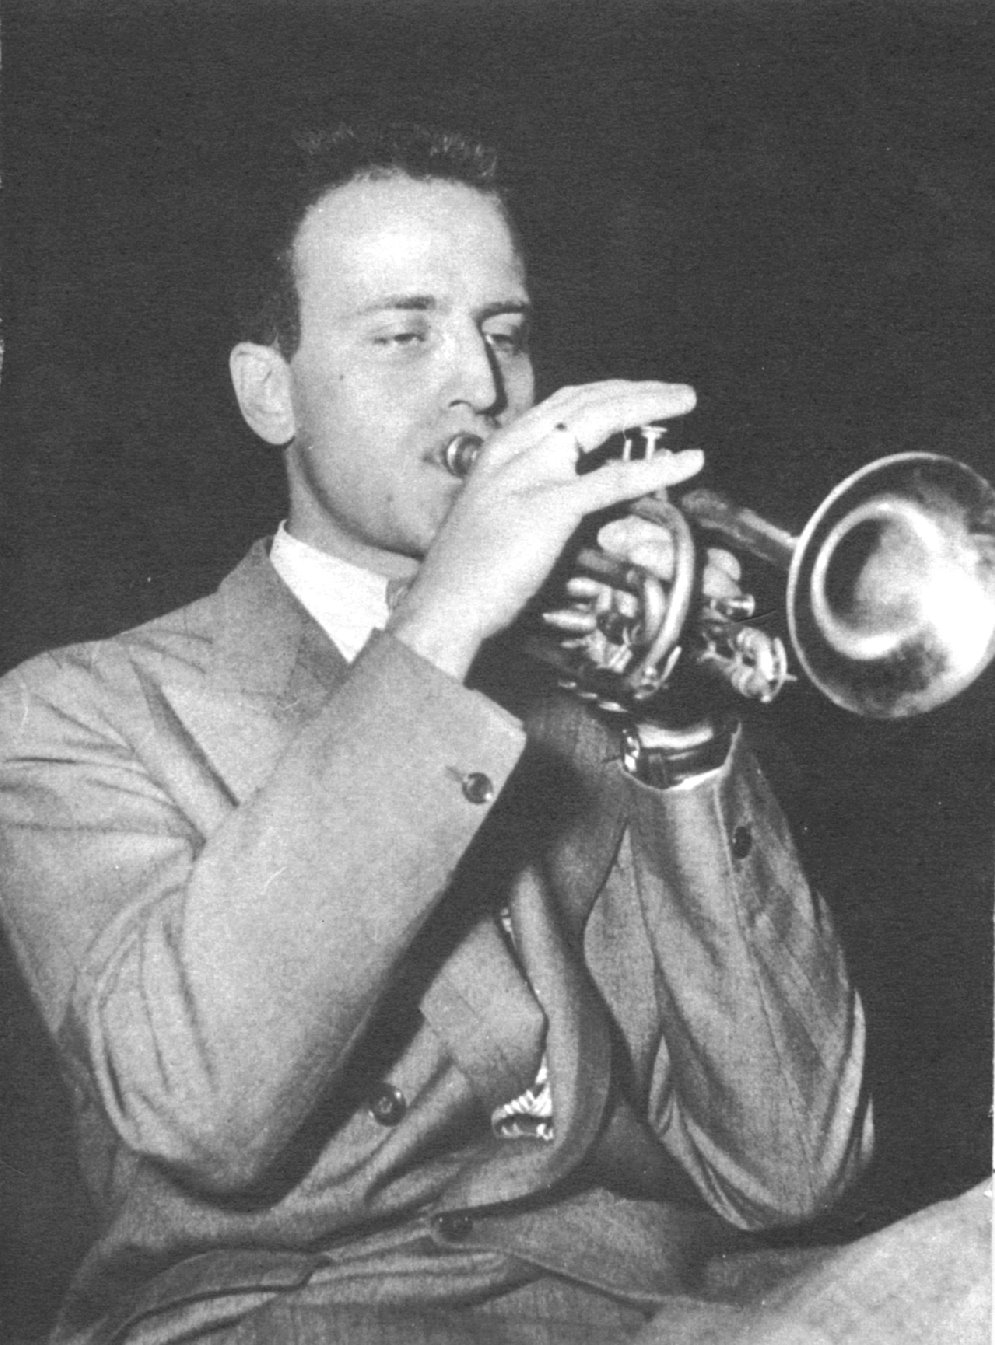
\includegraphics[width=\textwidth]{\PIXPATH/boris_trompette}
\caption{Boris jouant de sa trompinette}
\end{figure}

Il rejoint pendant quelque temps l'orchestre amateur
de Claude \bsc{Abadie}. Il est obligé d'arrêter à cause
de problèmes de santé.

Il passe alors à un autre domaine de la musique: parolier, puis interprète. Il est tellement
mauvais sur scène qu'il incite Serge  \bsc{Gainsbourg} à se lancer\ldots celui-ci se disant
que si Boris ose chanter sur scène comme cela, pourquoi pas lui. Il s'y est collé, non sans
un certain succès.

Avec Henri \bsc{Salvador}, qui deviendra vite son complice --- «Bobo et Salvaduch'» --- il
écrit les premiers rocks français.

Ce qui caractérise son approche de la musique --- quand il ne s'agit pas de faire de
l'alimentaire --- est «faut rigoler !»


\begin{figure}
\centering
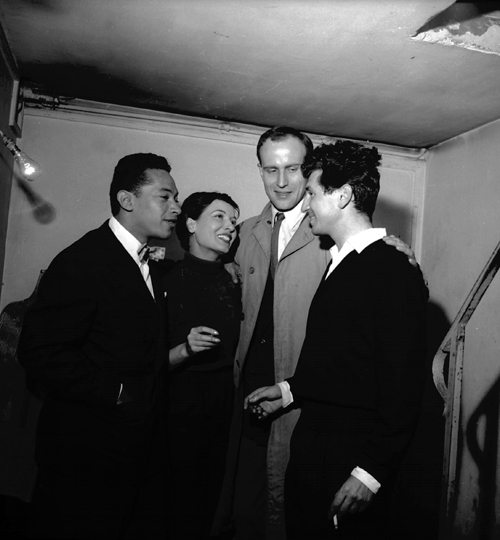
\includegraphics[width=\textwidth]{\PIXPATH/boris_gainsbourg}
\caption{Boris, Henri et Serge}
\end{figure}

\subsection{Le directeur artistique}

\section{Le Verbe}
\epigraph{Je me demande si je ne suis pas en train de jouer avec les mots. Et si les mots étaient faits pour ça ?}
{\emph{Les Bâtisseurs d'empire}, \BV}

\BV\ a manipulé les mots depuis sa plus tendre enfance. Les jeux de société à base
de ceux-ci étaient monnaie courante dans l'oisive vie vianesque vécue avant la mort
de Paul, le père.

\subsection{Écrits}

Sans doute le domaine où il aurait aimé être reconnu de son vivant, la littérature lui a apporté
ses plus grosses déceptions. En avance sur son temps, évoluant dans une société encore conservatrice,
il n'avait aucune chance. Ce n'est pas faute d'avoir essayé, pourtant. Mais, voyant que malgré tous
ses efforts personne ne voulait le publier, il passa à autre chose.

\subsubsection{L'écume}

C'est sans doute son roman le plus connu. Il fondait dessus beaucoup d'espoirs\~: quasi
assuré de gagner le prix de la Pléiade de la maison Gallimard (un honneur immense),
il a été sacrifié sur l'autel du conservatisme.

\subsubsection{J'irai cracher}

Écrit sous le pseudonyme de Vernon \bsc{Sullivan}, c'est au départ une blague\~: une fausse
traduction d'un roman américain. Réalisé pour dépanner un ami éditeur en manque de succès.
Fausse traduction écrite en quinze jours, mais vrai scandale, qui va poursuivre Boris
toute sa vie. Il devient célèbre après qu'un exemplaire ait été retrouvé, ouvert, sur une scène de crime.
Certes, le livre apporte des revenus substantiels, mais aussi des procès, qui
vont finir par faire censurer l'ouvrage.


Ce livre est très important dans la vie de \BV, car il va occulter ses «vrais» romans,
le discréditant auprès des autres écrivains et lui conférant une réputation sulfureuse
auprès du public. Boris va en souffrir tout le reste de sa vie.

\subsection{La 'Pataphysique}

Laissons Boris définir la 'Pataphysique, c'est encore ce qu'il y
a de plus simple\footnote{Tout est relatif !} et efficace.

{\small
\begin{quotation}
- Il semblerait que les pataphysiciens dont vous êtes, Satrape Boris Vian, l´un des plus étincelants fleurons, mettent tout leur sérieux à ne rien prendre au sérieux. Mais votre doctrine est si subtile et si vaste à la fois que certains de ses aspects peuvent échapper aux profanes que nous sommes. Peut-être pourriez-vous éclairer nos auditeurs avides de lumière sur le sens profond de la pataphysique\ldots Et nul n´est mieux qualifié que vous pour allumer notre lanterne. Nous vous écoutons dans le plus grand recueillement.

- Écoutez, la pataphysique est admirablement définie par Alfred Jarry dans les "Gestes et opinions du docteur Faustroll". Je crois que cette émission vous donnera d´ailleurs les définitions-mêmes de Jarry. Pour résumer les choses un peu simplement, on peut dire que la pataphysique est à la métaphysique ce que la métaphysique est à la physique. Un des principes fondamentaux de la pataphysique est d´ailleurs celui de l´équivalence des contraires. C´est peut-être ce qui vous explique ce refus que nous manifestons de ce qui est sérieux et de ce qui ne l´est pas, puisque pour nous, c´est exactement la même chose. C´est pataphysique. Qu´on le veuille ou qu´on ne le veuille pas, on fait toujours de la pataphysique

- Oui, sans le savoir

- Sans le savoir. Il est évident que plus la pataphysique est consciente, plus elle se double de pataphysique inconsciente parce que le fait-même de vouloir en faire est un acte hautement pataphysique. Et ce que l´on ignore lorsqu´on en fait volontairement est encore plus pataphysique peut-être. Si vous voulez qu´on donne un autre résumé, enfin, un autre principe, c´est l´intérêt que portent les pataphysiciens à l´exception plutôt qu´au cas général.Vous savez que Jarry considère les lois générales de la physique comme un ensemble d´exceptions non exceptionnelles et par conséquent sans aucun intérêt, l´exception exceptionnelle seule ayant un intérêt. Vous savez d´ailleurs que puisque, selon une autre formule, la pataphysique est la science, vous savez d´ailleurs qu´en sciences, il n´y a guère que l´exception qui fasse avancer ladite science. Je n´ai pas besoin de vous rappeler les exemples de Flemming, de Pasteur et de tous ces illustres savants pour que vous constatiez que la majeure partie...

- Toute découverte se fait par hasard

- Toute découverte se fait non seulement par hasard mais...

- C´est un faux pas

- C´est pas un faux pas, c´est le moment où l´observateur remarque une anomalie. C´est l´anomalie qui fait découvrir la découverte, si l´on peut employer ce pléonasme. C´est l´anomalie, c´est l´histoire de la culture de penicillium notatum de Flemming qui, grâce à Dieu et à Faulstroll surtout lui a fait prendre conscience...

- Oui, il me semblait bien en effet que Faustroll avait un rôle à jouer dans la découverte de la pénicilline mais vous faites bien de m´éclairer là-dessus

- Je me permets d´ajouter un dernier mot : Il n´y a pas besoin de s´attendre à des choses compliquées pour trouver la pataphysique. Pour vous donner un détail personnel, je suis venu à la pataphysique vers l´âge de huit ou neuf ans en lisant une pièce de Robert de Flers et de Caillavet qui s´appelle " La Belle Aventure ". C´est vraiment le dernier endroit où l´on peut s´attendre à en trouver quand on n´est pas pataphysicien. Mais elle contenait notamment cette réplique, qui était à la création dans la bouche de Victor Boucher et que je vous donne pour conclure ce petit entretien préalable; je crois qu´elle peut initier tout le monde très aisément et très rapidement à la pataphysique et c´est la suivante : " Je m´applique volontiers à penser aux choses auxquelles je pense que les autres ne penseront pas "

\end{quotation}
} 

Cette description de la 'Pataphysique, et la lecture de l'\oe{}uvre de \BV\ --- qui a très tôt été
confronté aux écrits de Jarry, le père de cette science --- montre que Boris a dû énormément
se plaire au sein du collège de 'Pataphysique. Jouer avec les mots et avec les
idées dans le seul but de jouer, que demander de mieux ? Il peut y exprimer tout
son savoir faire absurde et rhétorique.


\section*{Conclusion}

Cet aperçu, bien que rapide, incomplet et superficiel, montre tout de même des traits qui ont fait de \BV\ la
légende qu'il est devenu --- et qu'il était déjà de son vivant. Il a donné toute son énergie pour ses passions,
que ce soit le jazz ou les mots, et tant d'autres\~: ses amis, les voitures, le théâtre, l'opéra\ldots sans
oublier sa famille.

Mais il était gêné. Il traînait\footnote{Pas Charles, vous l'aurez compris. \BV\ appréciait beaucoup ce dernier.}
en lui la maladie qui allait le terrasser à \nb{39} ans seulement, laissant en plan tant de choses qu'il faisait,
et tant d'autres qu'il aurait aimé faire.

